% ============================ 1. VALUE CHAIN ==================================
\newpage
\setcounter{section}{0}
\phase{Section one}{The value chain, layer by layer}{Fifteen layers from sunlight to finance: who makes money in each, how much it costs to play, and how hard it is to get in.}

\subsection{The map}

\begin{figure}[H]
\centering
\begin{tikzpicture}[
  lay/.style={rounded corners=1.5pt,fill=#1,text=paper,align=center,font=\scriptsize\bfseries,minimum height=10mm,text width=19mm,inner sep=2pt},
  sup/.style={rounded corners=1.5pt,fill=wash,align=center,font=\scriptsize,minimum height=8mm,text width=19mm,inner sep=2pt},
  ar/.style={-{Stealth[length=2mm]},line width=0.8pt,color=ink2},
  gl/.style={font=\eyebrowfont\fontsize{5.8}{7}\selectfont,text=brass}]
\node[lay=sochre] (p) at (0,0) {1 Renewable power};
\node[lay=sblue] (s) at (2.55,0) {2 Electrolyser stacks};
\node[lay=ink2] (b) at (5.1,0) {5 Balance of plant};
\node[lay=sgreen] (d) at (7.65,0) {11 Ammonia, methanol, steel};
\node[lay=sviolet] (h) at (10.2,0) {12 Supply to customer (H\textsubscript{2}-as-a-service)};
\node[sup,below=4mm of s] (c) {3 Membranes, catalysts, electrodes};
\node[sup,below=2mm of c] (pe) {4 Power electronics};
\node[sup,below=4mm of b] (dev) {6 Development};
\node[sup,below=2mm of dev] (epc) {7 EPC (build)};
\node[sup,below=2mm of epc] (om) {8 O\&M and stack service};
\node[sup,below=4mm of d] (st) {9 Storage};
\node[sup,below=2mm of st] (tr) {10 Transport and cracking};
\node[sup,below=4mm of h] (cert) {13 Certification / MRV};
\node[sup,below=2mm of cert] (dig) {14 Digital: monitoring, trading};
\draw[ar] (p) -- (s); \draw[ar] (s) -- (b); \draw[ar] (b) -- (d); \draw[ar] (d) -- (h);
\draw[ar] (c) -- (s); \draw[ar] (dev.north) -- (b.south);
\draw[ar] (st.north) -- (d.south); \draw[ar] (cert.north) -- (h.south);
\node[rounded corners=1.5pt,fill=ink,text=paper,font=\scriptsize\bfseries,minimum width=122mm,minimum height=7mm] (fin) at (5.1,-4.15) {15 Financing: equity, project debt, development banks, subsidies};
\node[gl,above=1.5mm of p] {MAKE POWER};
\node[gl,above=1.5mm of s] {SPLIT WATER};
\node[gl,above=1.5mm of b] {BUILD};
\node[gl,above=1.5mm of d] {PRODUCT};
\node[gl,above=1.5mm of h] {CUSTOMER};
\end{tikzpicture}
\caption{The green hydrogen value chain. The top row is the physical flow; the boxes below each are the businesses that serve that step. Financing runs under everything.}
\end{figure}

\subsection{The economics of each layer}

Scores use the five-step scale from Dossier 1. Here, a 5 under \emph{capital intensity}, \emph{concentration} or \emph{barriers} means that column is high (usually bad for a newcomer); a 5 under \emph{growth} means fast growth to 2035 (good).

{\tablefont
\begin{xltabular}{\textwidth}{@{}>{\RaggedRight\arraybackslash}p{30mm} L c c c c@{}}
\caption{Value-chain economics. Margins are typical ranges with the anchor evidence named; scores are my judgement.}\\
\toprule
\thead{Layer} & \thead{Typical margin (evidence)} & \thead{Capital} & \thead{Concen.} & \thead{Barriers} & \thead{Growth}\\ \midrule
\endfirsthead
\toprule
\thead{Layer} & \thead{Typical margin (evidence)} & \thead{Capital} & \thead{Concen.} & \thead{Barriers} & \thead{Growth}\\ \midrule
\endhead
1 Renewable power & EBITDA 85–90\%: ACME Q4 FY25 90.5\% \cite{acmefy25} \rep; returns on capital far lower because assets are huge \estd & 5 & 3 & 4 & 5\\
2 Electrolyser stacks & Around zero or negative: nucera EBIT about €2m on €845m \cite{nucera2025}; Enapter EBITDA $-$€18.1m on €22.1m \cite{enapter2026} \rep & 4 & 5 & 4 & 2\\
3 Membranes, catalysts, electrodes & 20–40\% gross for incumbents with IP \estd & 3 & 5 & 5 & 3\\
4 Power electronics & 10–15\% EBITDA, like other industrial electrical kit \estd & 3 & 4 & 3 & 3\\
5 Balance of plant (water, compression, gas clean-up) & 8–15\% EBITDA \estd & 2 & 2 & 2 & 3\\
6 Project development & Lumpy: earned as a premium when a built, contracted plant is sold or financed \estd & 3 & 3 & 3 & 3\\
7 EPC (build) & 4–10\% EBITDA: Sterling \& Wilson FY25 about 4.6\% \cite{sw2025} \estd & 2 & 3 & 3 & 3\\
8 O\&M and stack service & 15–25\% EBITDA, typical of industrial service contracts \estd & 1 & 4 & 2 & 4\\
9 Storage & Utility-like regulated returns, once demand exists \estd & 5 & 2 & 4 & 2\\
10 Transport and cracking & Pipelines utility-like; shipping cyclical; cracking pre-commercial \estd & 5 & 3 & 5 & 2\\
11 Ammonia, methanol, green steel & Thin: SECI green ammonia averaged ₹53.27/kg, about 19\% above grey \cite{seci2025} \estd & 5 & 3 & 4 & 4\\
12 Supply to customer (H\textsubscript{2}-as-a-service) & About 30\%: Linde adjusted operating margin 29.8\% (FY2025) \cite{linde2026} \rep & 3 & 4 & 3 & 4\\
13 Certification / MRV & 20–40\% for verification services; software 60–80\% gross \estd & 1 & 3 & 3 & 4\\
14 Digital: monitoring, maintenance, trading & Software economics, 60–80\% gross once at scale \estd & 1 & 2 & 2 & 3\\
15 Financing & Lenders earn a 2–3\% spread; equity earns the residual \estd & 5 & 4 & 4 & 4\\
\bottomrule
\end{xltabular}}

\begin{figure}[H]
\centering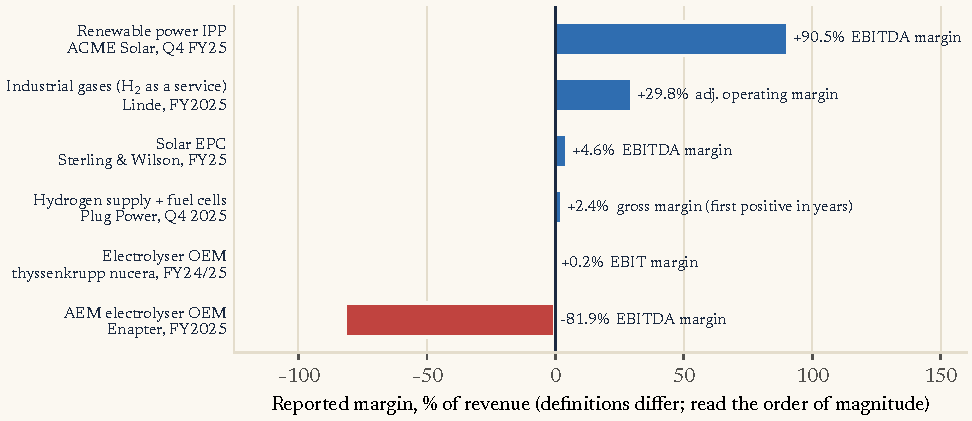
\includegraphics[width=\textwidth]{figures/profit_pools.pdf}
\caption{Profit pools in practice: one reported margin from each type of business. Sources: \cite{acmefy25,linde2026,sw2025,plug2026,nucera2025,enapter2026}. The EPC figure is my division of reported EBITDA by revenue.}
\end{figure}

\subsection{Who plays where}

Lists are illustrative, not exhaustive. Where I name a company without a citation, I am naming its line of business, not making a claim about its numbers.

{\tablefont
\begin{xltabular}{\textwidth}{@{}>{\RaggedRight\arraybackslash}p{24mm} L L L@{}}
\caption{Key players and growth signals by layer.}\\
\toprule
\thead{Layer} & \thead{India} & \thead{Global} & \thead{Growth signal (dated)}\\ \midrule
\endfirsthead
\toprule
\thead{Layer} & \thead{India} & \thead{Global} & \thead{Growth signal (dated)}\\ \midrule
\endhead
1 Power & ACME, Greenko, ReNew, Avaada, NTPC Renewable Energy & ACWA Power, Masdar, Iberdrola & Solar plus 4-hour storage at ₹2.86/kWh (Oct 2025) \cite{sqsolar2025} \rep\\
2 Stacks & Incentive winners: Reliance 300 MW, John Cockerill Greenko 300, Jindal India 300, Adani 198.5, Ohmium 137, Homihydrogen 101.5, Advait 100, L\&T 63 \cite{secipli2024} \rep & Peric, Longi, Sungrow (China); thyssenkrupp nucera, Nel, ITM, Siemens Energy; Electric Hydrogen & 58 GW/yr of factories ran at about 9\% in 2025 \cite{argus2026} \rep\\
3 Components & Newtrace (alkaline electrodes) \cite{newtrace2026} & Johnson Matthey, De Nora, Heraeus, Chemours & ITM cut iridium a further 40\% (Nov 2024) \cite{itm2024} \rep\\
4 Power electronics & Domestic power-equipment makers & ABB, Siemens, Hitachi Energy, Sungrow & Grows with every MW of electrolysis \estd\\
5 Balance of plant & Thermax, Ion Exchange & Atlas Copco, Burckhardt Compression & Desalination adds at most \usd{}0.10/kg \cite{rmi2023} \rep\\
6 Development & ACME, AM Green, Avaada, NTPC, Hygenco & ACWA Power, Air Products & 862,000 t/yr allocated, about 8,000 t/yr built \cite{sqnghm2025,chemindigest2026} \rep\\
7 EPC & L\&T, Tata Projects, Sterling \& Wilson & Technip Energies, Worley, Toyo & AM Green says all major contracts awarded (Jan 2026) \cite{amgreenuniper2026} \rep\\
8 O\&M, stacks & Mostly OEM service agreements; independents scarce & OEMs; industrial service firms & OEM distress: Cummins stopped selling electrolysers \cite{argus2026}; Enapter stack returns \cite{enapter2026} \rep\\
9 Storage & No large hydrogen storage; buffer tanks at plants & Salt caverns (US, Europe) & Depends on hydrogen trade emerging \estd\\
10 Transport & Port hubs at Kandla, Paradip, Tuticorin \cite{rw2025} & Ammonia carriers; cracking: Topsoe, Amogy \cite{amogy2025} & Exporters ship ammonia, so cracking happens at the importer's end \estd\\
11 Derivatives & AM Green, ACME, NTPC REL, Jakson, Onix, SCC, Oriana \cite{seci2025}; 5 steel pilots \cite{sqnghm2025} & Yara, CF Industries & Uniper to take up to 500,000 t/yr from AM Green from 2028 \cite{amgreenuniper2026} \prj\\
12 H\textsubscript{2}-as-a-service & Hygenco (Jindal Stainless, BOOT) \cite{hygenco2024}; Linde India, INOX Air Products & Linde, Air Liquide, Air Products & Industrial-gas margins near 30\% \cite{linde2026} \rep\\
13 Certification & BEE and accredited verification agencies under the 2025 certification scheme \cite{ghci2025} & DNV, TÜV, Bureau Veritas & EU buyers want RFNBO-certified ammonia \cite{amgreenuniper2026} \rep\\
14 Digital & Nascent; few hydrogen-specific players found & Siemens, AVEVA, Honeywell & Grows with plant count and certification rules \estd\\
15 Financing & REC (₹4,000 crore loan for ACME's Oman project) \cite{acmeodisha2023}; IREDA, PFC, SBI & World Bank (\usd{}1.5 bn for India's low-carbon transition) \cite{wb2023}; GIC, ADIA \cite{greenkogic2019} & Large balance sheets dominate; small tickets underserved \estd\\
\bottomrule
\end{xltabular}}

\subsection{Reading the map: margin against capital}

\begin{figure}[H]
\centering
\begin{tikzpicture}[x=1.15cm,y=0.95cm,
  dot/.style={circle,fill=#1,minimum size=5.2mm,inner sep=0,text=paper,font=\tiny\bfseries},
  ql/.style={font=\eyebrowfont\fontsize{6}{7}\selectfont,text=brass,align=center}]
\fill[sgreen!10] (0.5,3) rectangle (3,5.5); \fill[sochre!10] (3,3) rectangle (5.5,5.5);
\fill[wash] (0.5,0.5) rectangle (3,3); \fill[sred!8] (3,0.5) rectangle (5.5,3);
\draw[-{Stealth[length=2.5mm]},ink2,line width=0.8pt] (0.5,0.5) -- (5.8,0.5) node[right,font=\footnotesize,align=left,text=ink2] {capital\\ needed};
\draw[-{Stealth[length=2.5mm]},ink2,line width=0.8pt] (0.5,0.5) -- (0.5,5.8) node[above,font=\footnotesize,text=ink2] {margin a newcomer can earn};
\node[ql] at (1.75,5.25) {SWEET SPOT};
\node[ql] at (4.25,5.25) {RICH BUT CAPITAL-HUNGRY};
\node[ql] at (1.75,0.75) {SQUEEZED};
\node[ql] at (4.25,0.75) {VALUE TRAP};
\foreach \x/\y/\n/\c in {4.9/4.6/1/sochre, 4.1/1.1/2/sblue, 3.1/3.9/3/sblue, 3.0/2.6/4/ink2, 2.0/2.1/5/ink2, 3.2/2.9/6/ink2, 2.2/1.5/7/ink2, 1.4/3.9/8/sgreen, 4.9/2.0/9/ink2, 5.2/1.6/10/ink2, 4.8/2.4/11/sgreen, 3.3/4.3/12/sviolet, 1.2/4.4/13/sviolet, 1.0/3.5/14/sviolet, 4.6/3.4/15/ink}{
 \node[dot=\c] at (\x,\y) {\n};}
\end{tikzpicture}
\caption{My placement of the 15 layers (numbers match Table 1). Upper-left is where a capital-light newcomer can earn good margins.}
\end{figure}

\begin{finding}[Key finding \textbullet\ a smile curve, with a sweet spot near the customer]
The highest margins sit at the two ends: owning contracted power or contracted supply (layers 1, 12) and owning knowledge (layers 3, 13). Both ends are capital-hungry \emph{except} the knowledge end. The middle, making stacks and building plants (layers 2, 5, 7), is squeezed by Chinese overcapacity and reverse auctions. A newcomer without a balance sheet should aim for the upper-left: \textbf{O\&M and stack service (8), certification and MRV (13), digital (14), and a capital-light version of hydrogen-as-a-service (12)}. \confM
\end{finding}
